%\documentclass[mathserif]{beamer}
\documentclass[handout]{beamer}
%\usetheme{Goettingen}
\usetheme{Warsaw}
%\usetheme{Singapore}
%\usetheme{Frankfurt}
%\usetheme{Copenhagen}
%\usetheme{Szeged}
%\usetheme{Montpellier}
%\usetheme{CambridgeUS}
%\usecolortheme{}
%\setbeamercovered{transparent}
\usepackage[english, activeacute]{babel}
\usepackage[utf8]{inputenc}
\usepackage{amsmath, amssymb}
\usepackage{dsfont}
\usepackage{graphics}
\usepackage{cases}
\usepackage{graphicx}
\usepackage{pgf}
\usepackage{epsfig}
\usepackage{amssymb}
\usepackage{multirow}	
\usepackage{amstext}
\usepackage[ruled,vlined,lined]{algorithm2e}
\usepackage{amsmath}
\usepackage{epic}
\usepackage{epsfig}
\usepackage{fontenc}
\usepackage{framed,color}
\usepackage{palatino, url, multicol}
\usepackage{listings}
%\algsetup{indent=2em}
\newcommand{\factorial}{\ensuremath{\mbox{\sc Factorial}}}
\newcommand{\BIGOP}[1]{\mathop{\mathchoice%
{\raise-0.22em\hbox{\huge $#1$}}%
{\raise-0.05em\hbox{\Large $#1$}}{\hbox{\large $#1$}}{#1}}}
\newcommand{\bigtimes}{\BIGOP{\times}}
\vspace{-0.5cm}
\title{Introduction to Statistical Inference}
\vspace{-0.5cm}
\author[Felipe Bravo Márquez]{\footnotesize
%\author{\footnotesize  
 \textcolor[rgb]{0.00,0.00,1.00}{Felipe José Bravo Márquez}} 
\date{ \today }


\begin{document}
\begin{frame}
\titlepage


\end{frame}


%%%%%%%%%%%%%%%%%%%%%%%%%%%

% Useful references: http://www.buders.com/UNIVERSITE/Universite_Dersleri/istatistik/sampling_distributions_and_point_estimation_of_parameters.pdf
% http://homepage.divms.uiowa.edu/~rdecook/stat2020/notes/ch7_pt1.pdf

\begin{frame}{Populations and Samples}
\scriptsize{
\begin{itemize}
 \item The main goal of statistical inference is investigate properties about a target \textbf{population}.
 \item Example: What is the average height of the Chilean people? 
  \item In order to draw conclusions about a \textbf{population}, it is generally not feasible to gather all the data about it.
 \item We must make reasonable conclusions about a population based on the evidence provided by \textbf{sample data}.

 \item A \textbf{sample staticic} or simply \textbf{statistic} is a quantitative measure calculated from the data. Examples: the mean, the standard deviation, the minimum, the maximum.
 
 
 \item Our goal in sampling is to determine the value of a statistic for an entire population of interest, using just a small subset of the population.
 
 \item We do this primarily to save time and effort.
 
 \item Idea: Why go to the trouble of measuring every individual in the population when just a small sample is sufficient to accurately estimate the statistic of interest? \cite{poldrack2019statistical}
 
 

\end{itemize}

} 
\end{frame}


\begin{frame}{Samples and Surveys}
\scriptsize{
\begin{itemize}
 \item Random samples
 \item Stratified samples
 \item Biases

\end{itemize}

} 
\end{frame}


\begin{frame}{Statistical Inference }
\scriptsize{
\begin{itemize}
 \item The process of drawing conclusions about a population from sample data is known as \textbf{statistical inference}.
\item From a general point of view, the goal of inference is to \textbf{infer} the distribution that generates the observed data.
\item Example: Given a sample $X_1, \dots, X_n \sim F$, how do we infer $F$? 
\item However, in most cases we are only interested in inferring some property of $F$ (e.g., its \textbf{mean} value).
\item Statistical models that assume that the distribution can be modeled with a finite set of parameters $\theta= (\theta_{1},\theta_{2},\dots,\theta_{k})$ are called \textbf{parametric models}. 
\item Example: if we assume that the data comes from a normal distribution $N(\mu,\sigma^2)$, $\mu$ and $\sigma$ would be the parameters of the model. 
\end{itemize}

} 
\end{frame}


\begin{frame}{Frequentist Aproaches}
\scriptsize{
The satistical methods to be presented is this class are known as \textbf{frequentist (or classical)} methods. They are based on the following postulates  \cite{wasserman2013all}:
\begin{itemize}
\item Probability refers to limiting relative frequencies. Probabilities are objective properties of the real world.
\item Parameters are fixed, unknown constants. Because they are not fluctuating, no useful probability statements can be made about parameters.
\item Statistical procedures should be designed to have well-defined long run frequency properties. For example, a 95 percent confidence interval should trap the true value of the parameter with limiting frequency at least 95 percent.
\end{itemize}
There is another approach to inference called \textbf{Bayesian inference}, which is based on different posulates, to be discussed later in the course.

} 
\end{frame}

\section{Point Estimation}

\begin{frame}{Point Estimation}
\scriptsize{
\begin{itemize}
 \item Point estimation is the process of finding the \textbf{best guess} for some quantity of interest from a \textbf{statistical sample}.
 \item In a general sence, this quantity of interest could be a parameter in a parametric model, a CDF $F$, a probability density function $f$, a regression function $r$, or a prediction for a future value $Y$ of some random variable.
 \item In this class we will consider this quantity of interest as a \textbf{population parameter} $\theta$. 
  \item By convention, we denote a point estimate of $\theta$ by $\hat{\theta}$ or $\hat{\theta}_n$.
 \item It is important to remark that while $\theta$ is an unknown fixed value, $\hat{\theta}$  depends on the data and is therefore a random variable. 
 \item We need to bear in mind that the process of sampling is by definition a random experiment. 
 
\end{itemize}

} 
\end{frame}

\begin{frame}{Point Estimation}

%http://homepage.divms.uiowa.edu/~rdecook/stat2020/notes/ch7_pt1.pdf

\scriptsize{
\begin{block}{Formal Definition}
\begin{itemize}
 \item Let $X_1, \dots, X_n$ be $n$ IID data points  from some distribution  $F$.
 \item A point estimator $\hat{\theta}_n$  of a parameter $\theta$ is some function of $X_1, \dots, X_n$:
 \begin{displaymath}
 \hat{\theta}_n=g(X_1, \dots, X_n) 
 \end{displaymath}
 
\end{itemize}

 
\end{block}

\begin{itemize}
 \item The \textbf{bias} of an estimator is defined as: 
\begin{displaymath}
 \text{bias}(\hat{\theta}_n)=\mathbb{E}(\hat{\theta}_n)-\theta
\end{displaymath}
\item An estimator is unbiased if $\mathbb{E}(\hat{\theta}_n)=\theta$ or  $\text{bias}(\hat{\theta}_n)=0 $
\end{itemize}

} 
\end{frame}


\begin{frame}{Sampling Distribution}

\scriptsize{
% https://en.wikipedia.org/wiki/Sampling_distribution

\begin{itemize}
\item If we take multiple samples, the value of our statistical estimate $\hat{\theta}_n$ will also vary from sample to sample.

\item We refer to this distribution of our estimator across samples as the   \textbf{sampling distribution} \cite{poldrack2019statistical}.

\item The sampling distribution may be considered as the distribution of  $\hat{\theta}_n$ for all possible samples from the same population of size $n$\footnote{\url{https://courses.lumenlearning.com/boundless-statistics/chapter/sampling-distributions/}}.

\item The sampling distribution describes the variability of the point estimate around the true population parameter from sample to sample. 

\item We need to bear in mind this is an imaginary concept, since we can't obtain all possible samples.


\end{itemize}

} 
\end{frame}


\begin{frame}{Standard Error}

\scriptsize{

\begin{itemize}
\item The standard deviation of $\hat{\theta}_n$ is called the \textbf{standard error} $se$:
\begin{displaymath}
se(\hat{\theta}_n)=\sqrt{\mathbb{V}(\hat{\theta}_n})
\end{displaymath}
\item The standard error tells us about the variability of the estimator (and the sampling distribution) between all possible samples of the same size.
\item It is a measure of the uncertainty of the point estimate.
\end{itemize}

} 
\end{frame}





\begin{frame}{The Sample Mean}
\scriptsize{

\begin{itemize}
 \item Let $X_1,X_2,\dots,X_n$ be a random sample of a population of mean $\mu$ and variance $\sigma^2$.
 \item Let's suppose that we are interested in estimating $\mu$.
 \item  A sample statistic we can derive from the data is the  \textbf{sample mean} $\overline{X_{n}}$
 \begin{displaymath}
  \overline{X_{n}}=\frac{1}{n}\sum_{i=1}^{n} X_i
 \end{displaymath}
 \item The sample mean is an estimator of the mean $\overline{X_{n}} = \hat{\mu}$.

\item We can show that the sample mean is an unbiased estimator of $\mu$:
\begin{displaymath}
\mathbb{E}(\overline{X_{n}}) = \mathbb{E}(\frac 1n \sum_{i=1}^{n} X_i)  =  \frac 1n \times \mathbb{E}(\sum_{i=1}^{n} X_i) = \frac 1n (n \times \mu) = \mu  
\end{displaymath}
\end{itemize}

} 
\end{frame}

\begin{frame}{The Standard Error of the Sample Mean}
\scriptsize{

\begin{itemize}
\item The standard error of the sample mean $se(\overline{X_{n}}) = \sqrt{\mathbb{V}(\overline{X_{n}})}$ can be calulated as:
\begin{displaymath}
 \mathbb{V}(\overline{X_{n}})=\mathbb{V}(\frac 1n \sum_{i=1}^{n} X_i) = \frac{1}{n^2} \mathbb{V}(\sum_{i=1}^{n} X_i) = \frac{n}{n^2} \mathbb{V}(X_i)=\frac{\sigma^2}{n} 
\end{displaymath}

\item Then,  $se(\overline{X_{n}}) = \frac{\sigma}{\sqrt{n}}$

\end{itemize}


} 
\end{frame}




\begin{frame}{Sample and Population Variance}
\scriptsize{
\begin{itemize}
 \item  We usually do not know $\sigma$ of the population.
 \item When we want to estimate the variance of a population from a sample we are talking about the  \textbf{sample variance}:
\item The sample variance is defined as follows:

\begin{displaymath}
 s^{2}= \frac{1}{n-1} \sum_{i}^{n}(X_{i}-\overline{X_{n}})^2
\end{displaymath}

\item This is an unbiased estimator of the variance.

\item There is also the population variance (which is biased), defines as follows:

\begin{displaymath}
 s_{n}^{2}= \frac{1}{n} \sum_{i}^{n}(X_{i}-\overline{X_{n}})^2
\end{displaymath}

\item The population variance should only be calculated from population data (all the individuals), if is used as an estimator it would be biased.

\item The standard error of the sample mean when the population variance is unknown is estimated as follows:
\begin{displaymath}                                                                                                                 
\hat{se}(\overline{X_{n}}) = \frac{s}{\sqrt{n}}                                                                                                                \end{displaymath}


\end{itemize}


} 
\end{frame}



\begin{frame}[fragile]{The Sampling Distribution of the Sample Mean}
\scriptsize{

\begin{itemize}
\item Let us digress on the sampling distribution, which is a fundamental concept for understanding frequentist inference.
\item Imagine drawing (with replacement) all possible samples of size $n$ from a population.
\item Then for each sample, calculating a statistic--e.g., the sample mean. 
\item The frequency distribution of those sample means would be the sampling distribution of the mean (for samples of size $n$ drawn from that particular population).
\item Suppose, for example, that our population consisted of the following 5 scores: 2, 3, 4, 5, and 6. 
\item The population mean = 4, and the population standard deviation (dividing by N) = 1.414.

\end{itemize}

\begin{verbatim}

library(gtools)
library(tidyverse)
sd.p=function(x){sd(x)*sqrt((length(x)-1)/length(x))}

pop <-c(2,3,4,5,6)
samp_size <- 2

mean(pop)
sd.p(pop)

samples<-as_tibble(permutations(length(pop), samp_size, pop, repeats.allowed=TRUE))

samples <- samples %>% rowwise() %>% mutate(sample_mean=mean(c(V1,V2)))
 
\end{verbatim}


} 
\end{frame}


\begin{frame}{Point Estimation of a Proportion}
\scriptsize{
\begin{itemize}
 \item Let $X_1, \dots, X_n \sim$ Bernoulli$(p)$ and let $\hat{p}_{n}=\frac 1n \sum_{i}X_{i}$
 \item Then $\mathbb{E}(\hat{p}_{n})= \frac 1n \sum_i \mathbb{E}(X_i)=p$, and $\hat{p}_n$ is unbiased.
 \item The standard error $se$ would be
\begin{displaymath}
se = \sqrt{\mathbb{V}(\hat{p}_n)}= \sqrt{p(1-p)/n} 
\end{displaymath}
\item The estimated standard error $\hat{se}$:
\begin{displaymath}
\hat{se} =\sqrt{\hat{p}(1-\hat p)/n} 
\end{displaymath}

\end{itemize}


} 
\end{frame}




\begin{frame}{Consistency}

\scriptsize{

\begin{itemize}
\item A good estimator is expected to be unbiased and of minimum variance.

\item Unbiasedness used to receive much attention but these days is considered less important

\item Many of the estimators we will use are biased. 

\item A reasonable requirement for an estimator is that it should converge to the true parameter value as we collect more and more data.

\item A point estimator $\hat{\theta}_n$ of a parameter $\theta$ is \textbf{consistent}  if it converges to the true value when the number of data in the sample tends to infinity..
\item The quality of an estimator can be measured using the  \textbf{mean squared error} (MSE)
\begin{displaymath}
MSE = \mathbb{E}_{\theta}(\hat{\theta}_n - \theta)^2 
\end{displaymath}

\end{itemize}

} 
\end{frame}



\begin{frame}{Consistency}

\scriptsize{

\begin{itemize}
\item If for an estimator $\hat{\theta}_n$, its $bias \rightarrow 0$ and its $se \rightarrow 0$ when $n\rightarrow \infty$, $\hat{\theta}_n$, it is a consistent estimator of $\theta$.

\item For example, for the sample mean $\mathbb{E}(\overline{X_{n}})=\mu$ hich implies that the $bias =0$ and$se(\overline{X_{n}}) = \frac{\sigma}{\sqrt{n}}$  tends to zero when $n\rightarrow \infty$. Then $\overline{X_{n}}$ is a consistent estimator of the mean.  

\item For the case of the Bernoulli experiment one has that  $\mathbb{E}(\hat{p})=p \Rightarrow bias=0$ y $se = \sqrt{p(1-p)/n} \rightarrow 0$ when $n\rightarrow \infty$. Then  $\hat{p}$ is a consistent estimator of $p$.


\end{itemize}

} 
\end{frame}


\begin{frame}{Maximum Likelihood Estimation}
 
\end{frame}



\begin{frame}{Confidence Interval}
\scriptsize{
\begin{itemize}
 \item We know that the value of a point estimator \textbf{varies} from sample to sample.
 \item It is more reasonable to find an interval that is likely to trap the real value of the parameter with a certain probability.
 \item The general form of a confidence interval in the following:
  \begin{displaymath}
   \text{Confidence Interval} = \text{Sample Statistic} \ \pm \ \text{Margin Error}
  \end{displaymath}
 \item The wider the interval the more uncertainty there is about the value of the parameter.
\end{itemize}


}
 
\end{frame}


\begin{frame}{Confidence Interval }
\scriptsize{

\begin{block}{Definition}
\begin{itemize}
 \item A \textbf{confidence interval} for an unknown population parameter $\theta$ with a \textbf{confidence level} $1-\alpha$, is an interval $C_n = (a,b)$ where:
 \begin{displaymath}
 \mathbb{P}(\theta \in C_n) = 1-\alpha
\end{displaymath}
 \item In addition $a= a(X_1, \dots, X_n)$ and $b=b(X_1,\dots,X_n)$ are functions of the data.
 \item The $\alpha$ value is known as the \textbf{significance} level, generally taken as $0.05$, which is equivalent to working with a confidence level of $95\%$.
 \item Significance can be interpreted as the probability of being wrong.
\end{itemize}

\end{block}

}
 
\end{frame}


\begin{frame}{Confidence Interval}
\scriptsize{


\begin{itemize}
 \item There is a lot of \textbf{confusion} about how to interpret a confidence interval.
 \item A confidence interval is not a probability statement about $\theta$ since $\theta$ is a fixed quantity in Frequentist inference setting, not a random variable
 \item One way to interpret them is to say that if we repeat the \textbf{same experiment} many times, the interval will contain the value of the parameter $(1-\alpha)\%$ of the times.
 \item This interpretation is correct, but we rarely repeat the same experiment several times.
 \item A better interpretation: one day I collect data I create a $95\%$ confidence interval for a parameter $\theta_1$. Then on day 2, I do the same for a parameter $\theta_2$ and so repeatedly $n$ times. The $95\%$ of my intervals will contain the actual values of the parameters. 
 
\end{itemize}



}
 
\end{frame}




\begin{frame}{Confidence Interval}
\scriptsize{


\begin{itemize}
 \item Later in the course, we will discuss Bayesian methods in which we treat $\theta$ as if it were a random variable and we do make probability statements about $\theta$.
\item In particular, we will make statements like ``the probability that $\theta$  is in $C_n$, given the data, is 95 percent.''
\item However, these Bayesian intervals refer to degree-of-belief probabilities. 
\item These Bayesian intervals will not, in general, trap the parameter 95 percent of the time.
 
\end{itemize}



}
 
\end{frame}


\begin{frame}{Confidence Interval of the Mean }
\scriptsize{
\begin{itemize}
 \item We have $n$ independent observations $X_1, \dots, X_n$ (IID) of distribution $N(\mu,\sigma^2)$.
\item Suppose $\mu$ is \textbf{unknown} but $\sigma^2$ is \textbf{known}.
 \item We know that $\overline{X_{n}}$ is an unbiased estimator of $\mu$.
 \item By the law of large numbers we know that the distribution of $\overline{X_{n}}$ is concentrated around $\mu$ when $n$ is large.
 \item By the CLT we know that \begin{displaymath}
 Z=\frac{\overline{X_{n}}-\mu}{\frac{\sigma}{\sqrt{n}}}  \sim N(0,1)
\end{displaymath}
when $n$ is large.
\end{itemize}


 }
\end{frame}

\begin{frame}{Confidence Interval}
\scriptsize{
\begin{itemize}
 \item We want to find an interval $C_n = (\mu_1,\mu_2)$ with confidence level $1-\alpha$:
\begin{displaymath}
 \mathbb{P}(\mu_1 \leq \mu \leq \mu_2 ) = 1-\alpha
\end{displaymath}
\item Let $z_a = \Phi^{-1}(1-a)$, with $a \in [0,1]$ where $\Phi^{-1}$ is the quantile function of a standardized normal.
\item This is equivalent to saying that $z_a$ is the value such that $1-\Phi(z_a)=\mathbb{P}(Z \geq z_a)=a$.

\item By symmetry of the normal distribution: $z_{\alpha/2}=-z_{(1-\alpha/2)}$.
\end{itemize}


 }
\end{frame}



\begin{frame}{Confidence Interval}


\begin{figure}[h!]
	\centering
	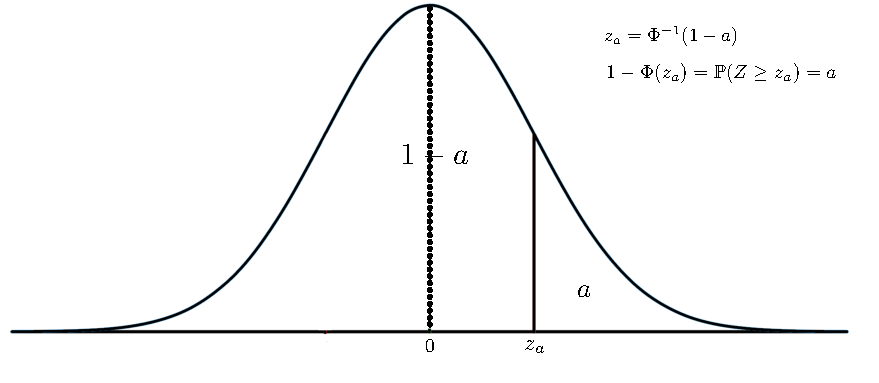
\includegraphics[scale=0.8]{pics/conf_int_1.pdf}
\end{figure}


 
\end{frame}


\begin{frame}{Confidence Interval}


\begin{figure}[h!]
	\centering
	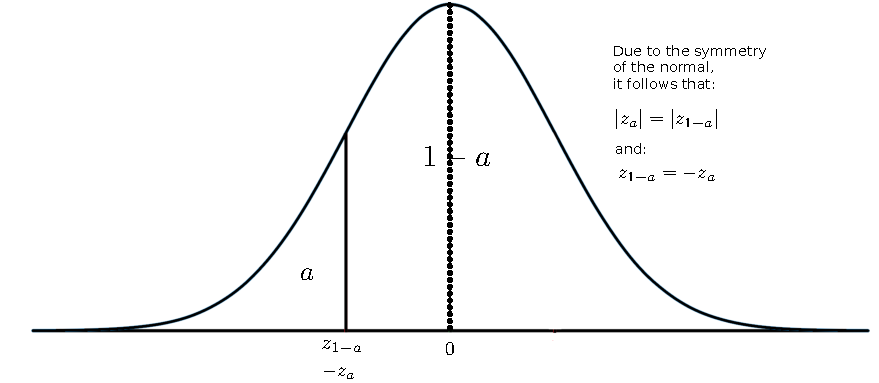
\includegraphics[scale=0.8]{pics/conf_int_2.pdf}
\end{figure}


 
\end{frame}


\begin{frame}{Confidence Interval}


\begin{figure}[h!]
	\centering
	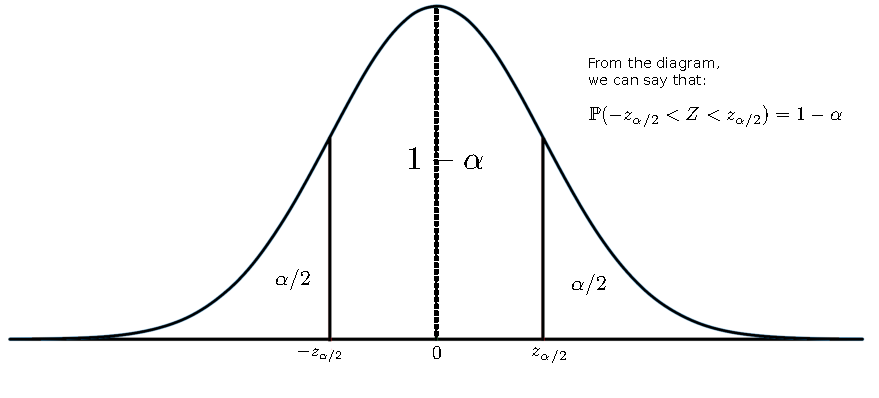
\includegraphics[scale=0.8]{pics/conf_int_3.pdf}
\end{figure}


 
\end{frame}


\begin{frame}{Confidence Interval}
\scriptsize{
\begin{itemize}
 \item  The confidence interval for $\mu$ is:
 \begin{displaymath}
 C_n = (\overline{X_{n}}-z_{\alpha/2}\frac{\sigma}{\sqrt{n}} , \overline{X_{n}} + z_{\alpha/2}\frac{\sigma}{\sqrt{n}}) 
 \end{displaymath}
\item Then $ z_{\alpha/2}$ tells us how many times we have to multiply the \textbf{standard error} to build the interval.
\item The smaller the value of $\alpha$ the larger the value of $ z_{\alpha/2}$ and hence the wider the interval.  
\item Proof:
 \begin{eqnarray*}
 \mathbb{P}(\mu \in C_n) & = & \mathbb{P}(\overline{X_{n}}-z_{\alpha/2}\frac{\sigma}{\sqrt{n}} < \mu < \overline{X_{n}} + z_{\alpha/2}\frac{\sigma}{\sqrt{n}}) \nonumber \\ 
                         & = & \mathbb{P}(-z_{\alpha/2} < \frac{\overline{X_{n}}-\mu}{\frac{\sigma}{\sqrt{n}}} <  z_{\alpha/2}) \nonumber \\ 
			  & = & \mathbb{P}(-z_{\alpha/2} < Z <  z_{\alpha/2}) \nonumber \\
			   & = & 1-\alpha 
 \end{eqnarray*}


\end{itemize}
}


 
\end{frame}

\begin{frame}[fragile]{Confidence Interval}

\scriptsize{
\begin{itemize}
 \item Since $z_{\alpha/2} = \Phi^{-1}(1-\alpha/2)$ we can use the quantile function of the normal to calculate confidence intervals in R.
\end{itemize}


\begin{verbatim}
> alpha <- 0.05
> xbar <- 5
> sigma <- 2
> n <- 20
> se <-sigma/sqrt(n)
> error <- qnorm(1-alpha/2)*se
> left <- xbar-error
> right <- xbar+error
> left
[1] 4.123477
> right
[1] 5.876523
>
\end{verbatim}
}



\end{frame}

\begin{frame}{T Distribution}
\scriptsize{
\begin{itemize}
 \item In practice, if we do not know $\mu$ we are unlikely to know $\sigma$.
 \item If we estimate $\sigma$ using $s$, confidence intervals are better build using the distribution \textbf{T-student}, especially when the sample size is small.
\end{itemize}

\begin{block}{T Distribution}
\begin{itemize}
 \item An R.V. has distribution $t$ with $k$ degrees of freedom when it has the following PDF:
\begin{displaymath}
 f(t)=\frac{\Gamma(\frac{k+1}{2})}{\sqrt{k\pi}\Gamma(\frac k2)(1+\frac{t^2}{k})^{(k+1)/2}}
\end{displaymath}
\item  When $k=1$ it is called \textbf{Cauchy} distribution.
\item When $k\rightarrow \infty$ it converges to a standardized normal distribution.
 \item The t-distribution has wider tails than the normal distribution when it has few degrees of freedom.


\end{itemize}

 
\end{block}




} 
\end{frame}

\begin{frame}[fragile]{T Distribution}
 \scriptsize{



\begin{verbatim*}
x<-seq(-8,8,length=400)
y1<-dnorm(x)
y2<-dt(x=x,df=1)
y3<-dt(x=x,df=10)
y4<-dt(x=x,df=350)
plot(y1~x,type="l",col="green")
lines(y2~x,type="l",col="blue")
lines(y3~x,type="l",col="black")
lines(y4~x,type="l",col="red")

\end{verbatim*}

 \begin{figure}[h!]
	\centering
	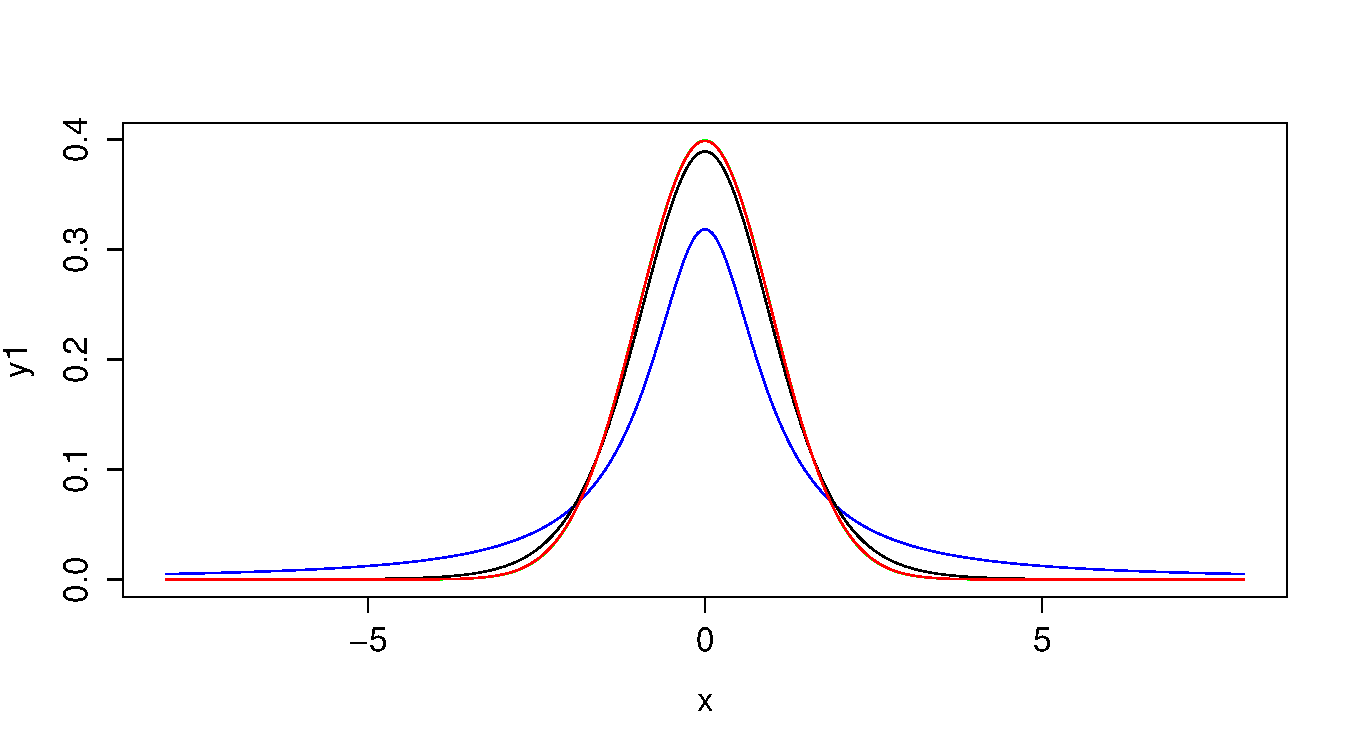
\includegraphics[scale=0.3]{pics/tstudent.pdf}
\end{figure}


}
\end{frame}


\begin{frame}{T-Distribution Confidence Interval}

\scriptsize{
\begin{itemize}
 \item Let  $s^{2}= \frac{1}{n-1} \sum_{i}^{n}(X_{i}-\overline{X_{n}})^2$ we have:
 \begin{displaymath}
  T=\frac{\overline{X_{n}}-\mu}{\frac{s}{\sqrt{n}}}\sim t_{n-1}
 \end{displaymath}
\item  Let $t_{n-1,a}=\mathbb{P}(T>a)$, equivalent to the quantile function $qt$ evaluated at $(1-a)$.
\item The resulting confidence interval is:
       \begin{displaymath}
 C_n = (\overline{X_{n}}-t_{n-1,\alpha/2}\frac{s}{\sqrt{n}} , \overline{X_{n}} + t_{n-1,\alpha/2}\frac{s}{\sqrt{n}}) 
 \end{displaymath} 
 \item Since the tails of the $t$ distribution are wider when $n$ is small, the resulting confidence intervals are wider.

\end{itemize}


}

\end{frame}


\begin{frame}[fragile]{T-Distribution Confidence Interval}
\scriptsize{
\begin{itemize}
 \item Let's calculate a confidence interval for the mean of \verb+Petal.Length+ of the \textbf{Iris} data with $95\%$ confidence.
\begin{verbatim}
>data(iris)
>alpha<-0.05
>n<-length(iris$Petal.Length)
>xbar<-mean(iris$Petal.Length)
>xbar
[1] 3.758
>s<-sd(iris$Petal.Length)
>se<-s/sqrt(n)
>error<-qt(p=1-alpha/2,df=n-1)*se
>left<-xbar-error
>left
[1] 3.473185
>right<-xbar+error
>right
[1] 4.042815
\end{verbatim}
\item Another way:
\begin{verbatim}
>test<-t.test(iris$Petal.Length,conf.level=0.95)
>test$conf.int
[1] 3.473185 4.042815
\end{verbatim}


\end{itemize}



}
 
\end{frame}

\begin{frame}{The Boostrap}
 
\end{frame}





%%%%%%%%%%%%%%%%%%%%%%%%%%%
%%%%%%%%%%%%%%%%%%%%%%%%%%%
\begin{frame}[allowframebreaks]\scriptsize
\frametitle{References}
\bibliography{bio}
\bibliographystyle{apalike}
%\bibliographystyle{flexbib}
\end{frame}  









%%%%%%%%%%%%%%%%%%%%%%%%%%%

\end{document}
